\section{Aufbau und Durchführung des Versuchs}
\subsection{Grundsätzliches Konzept des Aufbaus}
Der grundsätzliche Aufbau des Interferometers ist in Abbildung \ref{fig:interferometer_aufbau} dargestellt.
\begin{figure}[h!]
  \centering
  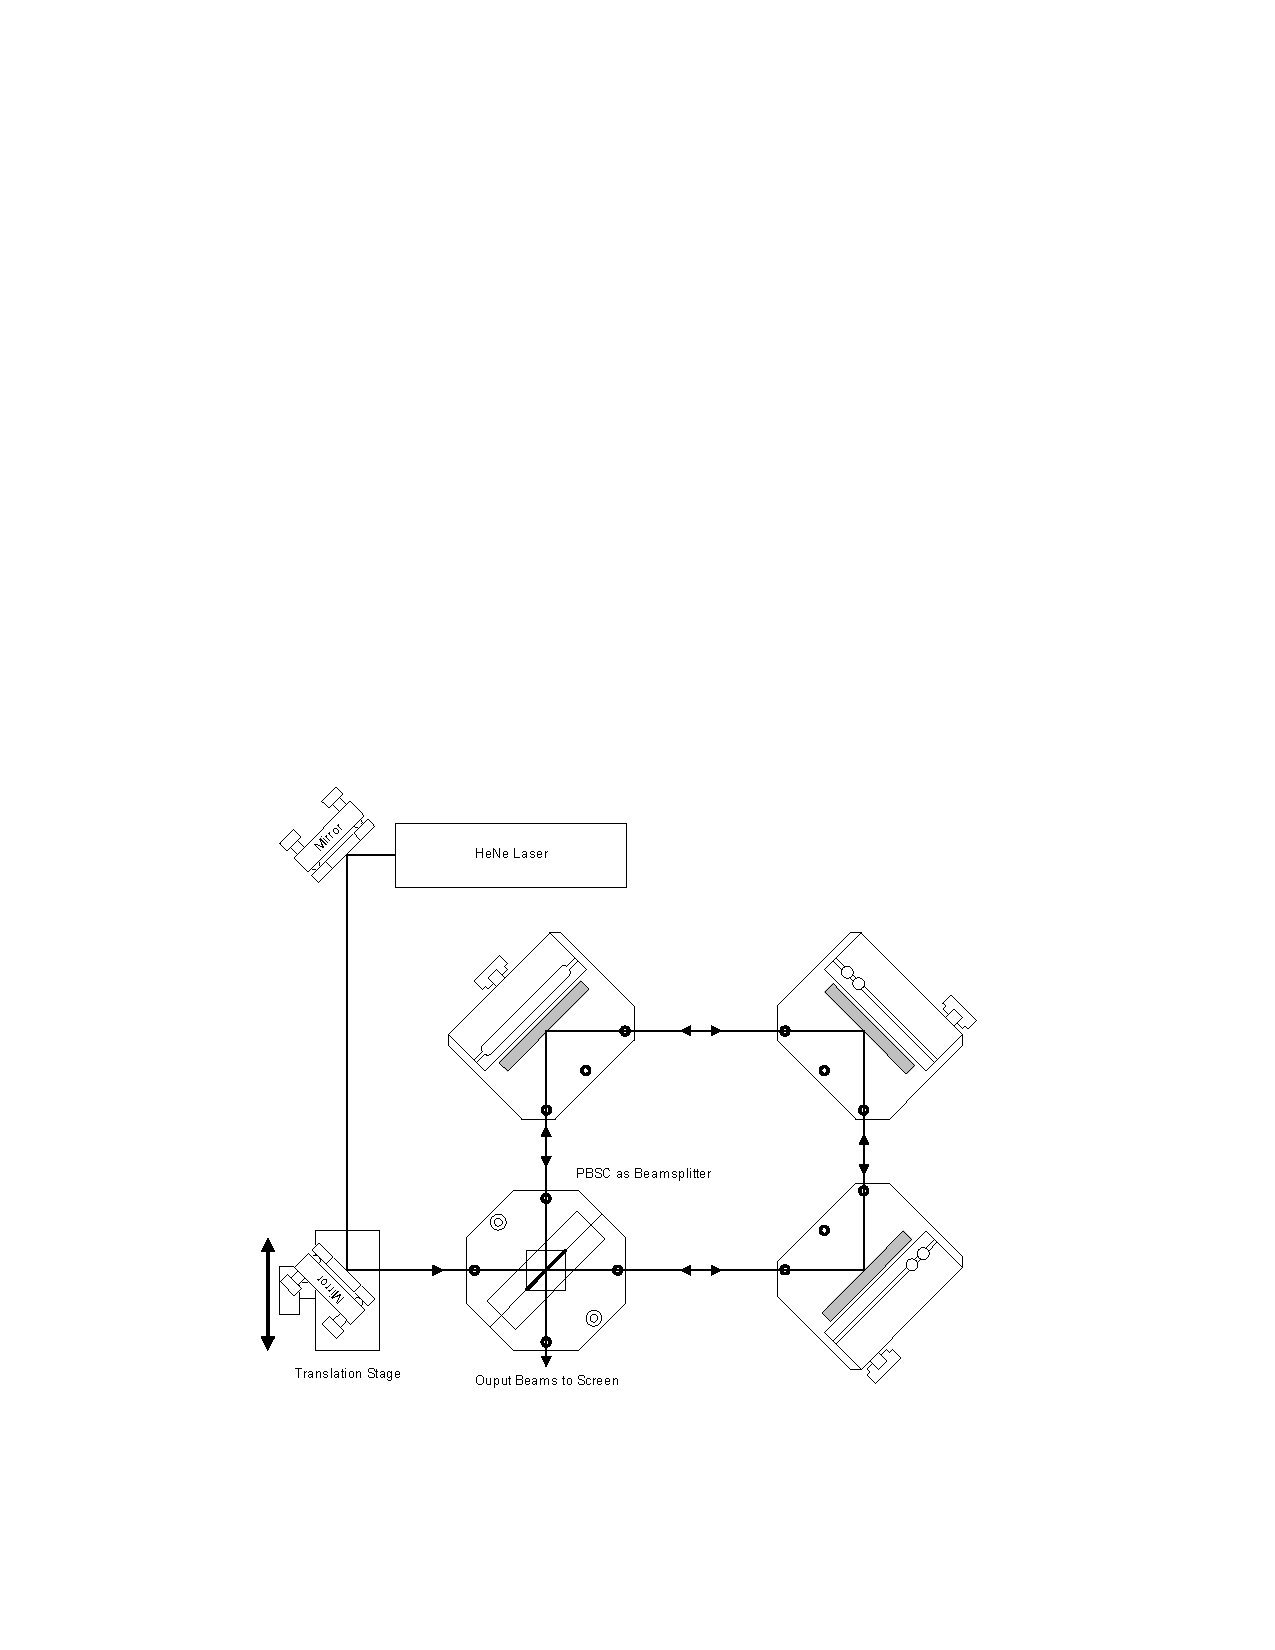
\includegraphics[width=0.85\textwidth]{content/images/interferometer_aufbau.pdf}
  \caption{Der konzeptionelle Aufbau des Interferometers \cite{teachspin}.}
  \label{fig:interferometer_aufbau}
\end{figure}
Der \texttt{Helium-Neon-Laser} gibt einen monochromatischen, roten Laserstrahl mit der Wellenlänge $\lambda = \SI{632.990}{nm}$ \cite{anleitung} aus.
Über zwei Spiegel wird der Strahl durch einen \texttt{linearen Polarisationsfilter} zum \texttt{PBSC} (eng. \textit{Polarising Beam Splitter Cube}) umgelenkt (Abb. \ref{fig:int_pbsc}).
Der PBSC (Abb. \ref{fig:pbsc}) ist ein Würfel, der durch eine dieelektrische Schicht diagonal in zwei Prismen geteilt wird.
Die s-polarisierte Komponente des Laserstrahls wird am Dielektrikum reflektiert, die p-polarisierte Komponente wird transmittiert.
\begin{figure}[h!]
  \centering
  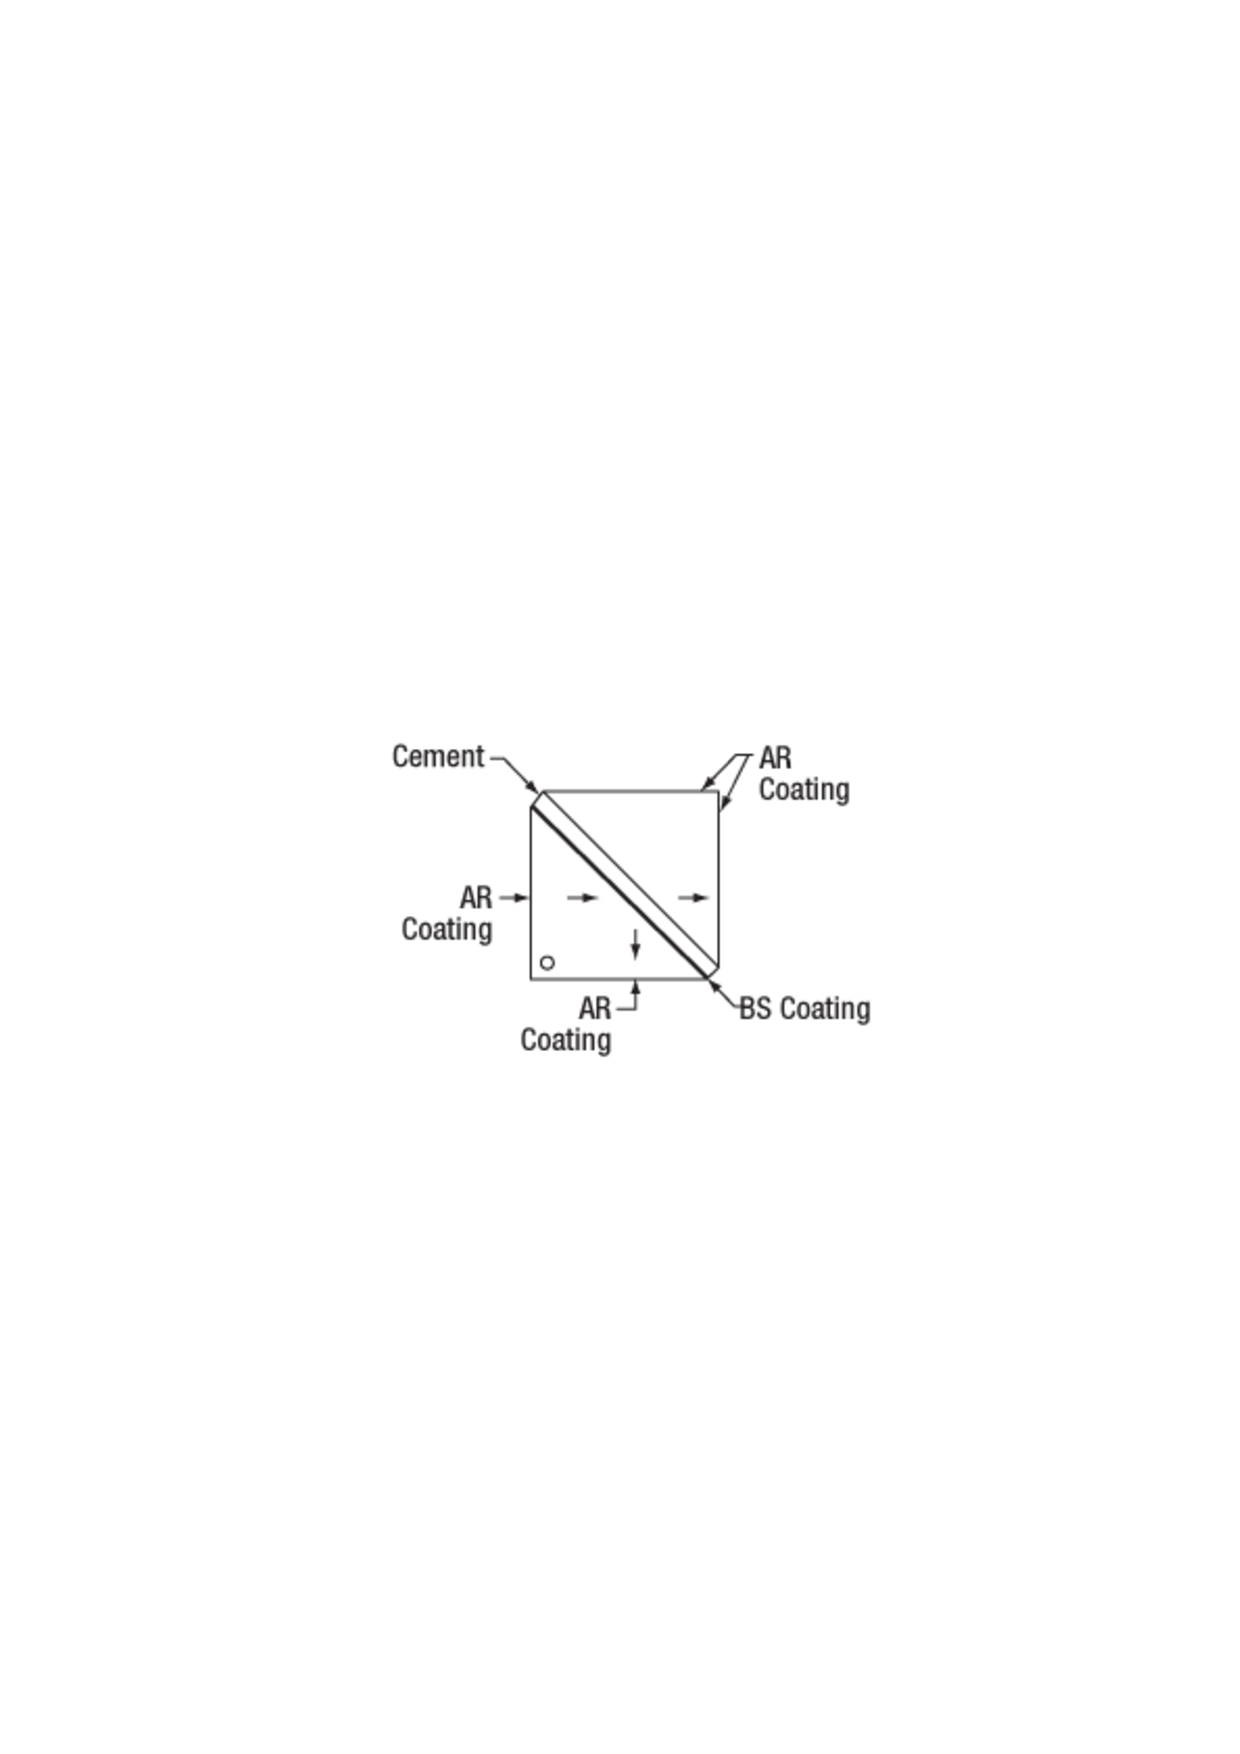
\includegraphics[width=0.35\textwidth]{content/images/pbsc.pdf}
  \caption{Prinzip eines \textit{Polarising Beam Splitter Cube} \cite{thorlabs}.}
  \label{fig:pbsc}
\end{figure}
Die verschieden polarisierten Teilstrahlen durchlaufen den Spiegelaufbau des Interferometers nun in gegensätzliche Richtungen (Abb. \ref{fig:int_mirr}).
\begin{figure}[!ht]
\begin{subfigure}[c]{0.50\textwidth}
    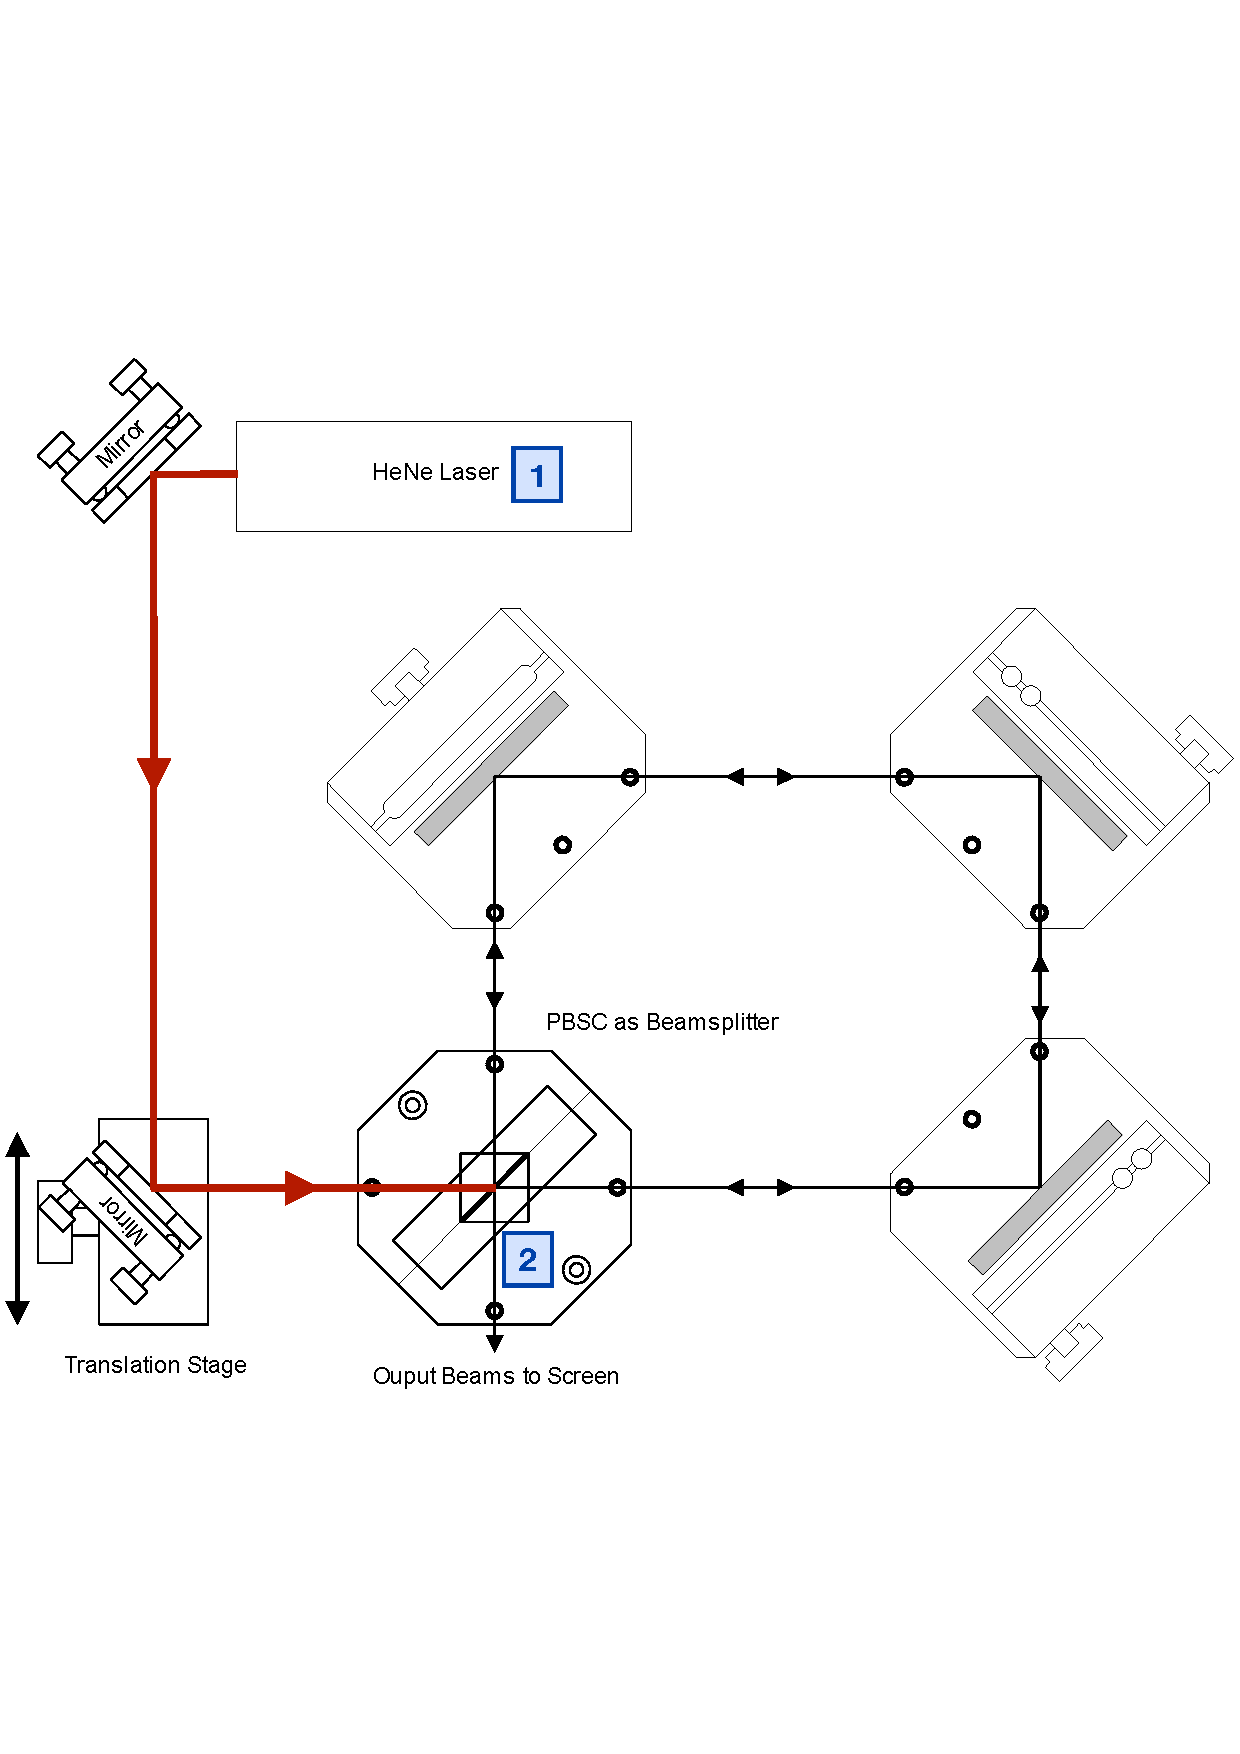
\includegraphics[width=\textwidth]{content/images/interferometer_1.pdf}
    \caption{Strahlengang bis zum PBSC (\cite{teachspin}, modifiziert).}
	\label{fig:int_pbsc}
\end{subfigure}
\hspace*{\fill}
\begin{subfigure}[c]{0.50\textwidth}
    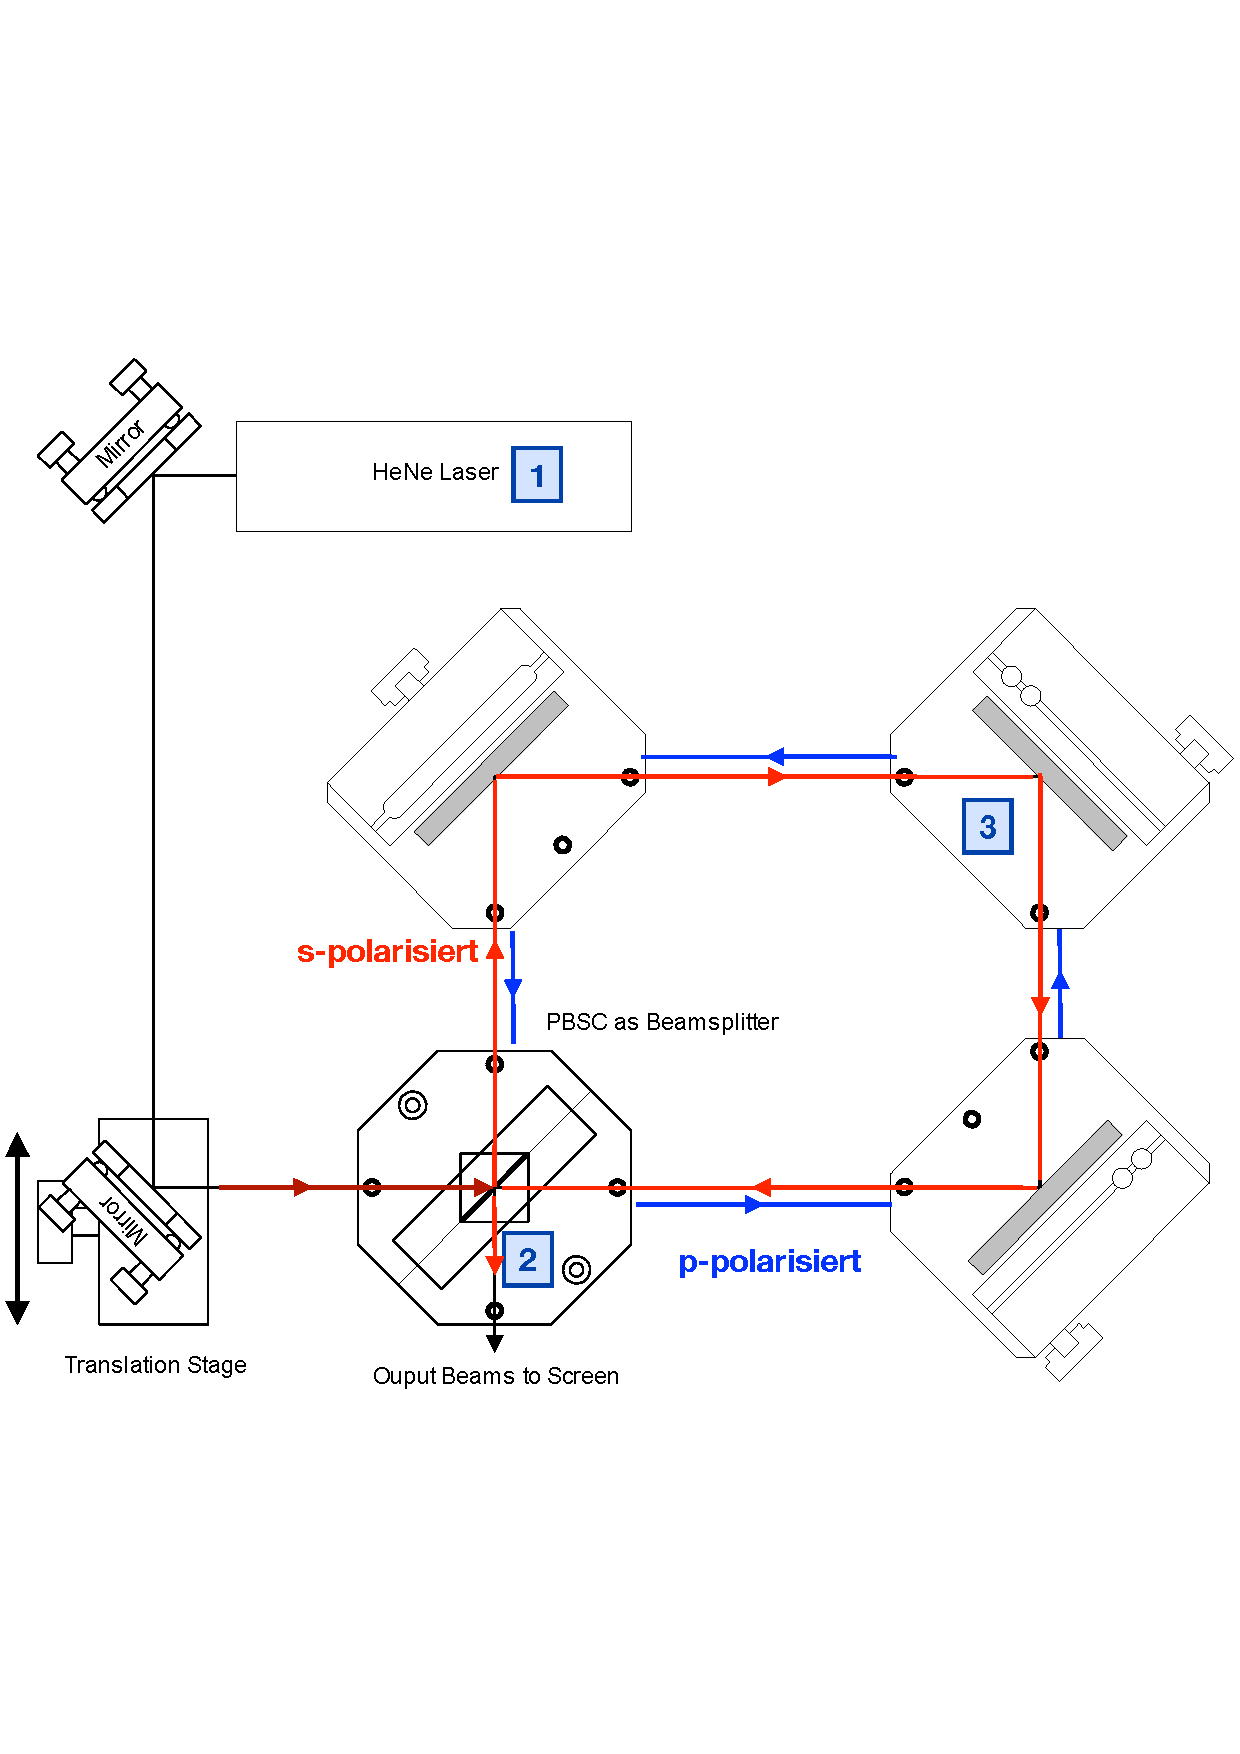
\includegraphics[width=\textwidth]{content/images/interferometer_2.pdf}
    \caption{Strahlengänge der verschiedenen Polarisationen bis zum Ausgang des Interferometers (\cite{teachspin}, modifiziert).\\
	\small{Zur Veranschaulichung sind die richtungsweisenden Pfeile der beiden Polarisationen nicht überlappend dargestellt, in Realität und bei optimaler Justage verlaufen beide Strahlengänge zunächst auf der gleichen Linie.}}
	\label{fig:int_mirr}
\end{subfigure}
%\caption{Verlauf des Strahlengang.}
\end{figure}
Die polarisierten Teilstrahlen werden beim zweiten Durchgang durch den PBSC wieder zu einem Strahl vereinigt.
Wird der zweite Spiegel im justierten Aufbau senkrecht zum ersten Polarisationsfilter verschoben, werden die beiden gegenläufigen Strahlen im Interferometer durch die Geometrie des Aufbaus getrennt, laufen aber trotzdem am Ende wieder zu einem Strahl zusammen (Abb. \ref{fig:int_teil}).
\begin{figure}[h!]
  \centering
  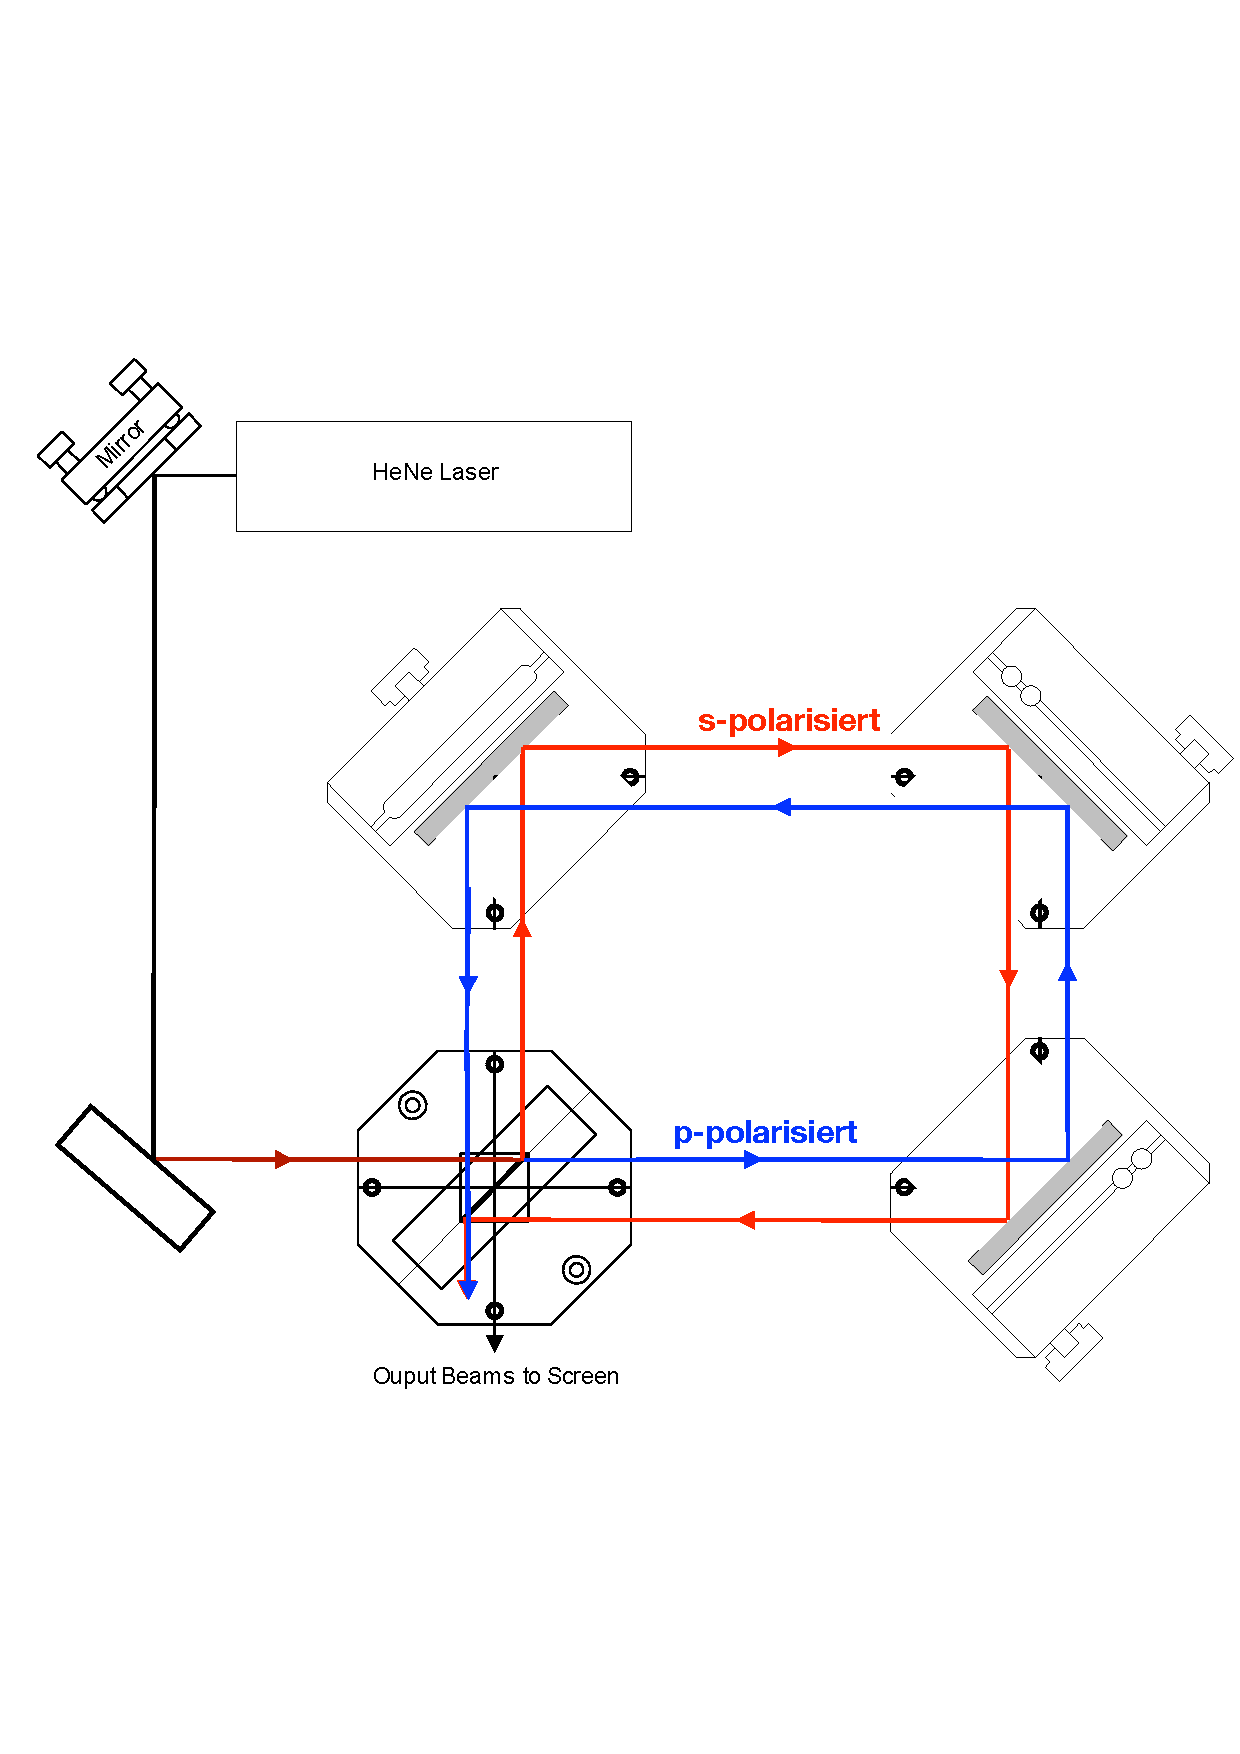
\includegraphics[width=0.85\textwidth]{content/images/interferometer_teil.pdf}
  \caption{Strahlengang der separierten Teilstrahlen im Sagnac-Interferometer  (\cite{teachspin}, modifiziert).}
  \label{fig:int_teil}
\end{figure}
Nach dem Durchgang durch das Interferometer wird, je nach Messung, der Strahl direkt auf einem Schirm abgefangen, oder er läuft weiter durch einen zweiten PBSC, der beide Polarisationen erneut separiert und auf zwei Photodioden projeziert.
\FloatBarrier

\subsection{Durchführung}
\paragraph{Justage}
Zur Justage wird der Strahlengang des Lasers zwischen den einzelnen Komponenten des Interferometers mit zwei Justageplatten (Platten mit Bohrung auf Höhe des Lasers) überprüft.
Direkt hinter dem PBSC wird einer der beiden Teilstrahlen unterbrochen, während der Strahlengang des anderen Teilstrahls untersucht wird.
Zunächst wird die Ausrichtung und Höhe der Komponenten auf der Bodenplatte angepasst und die Komponenten werden fest geschraubt, so dass der Laser die Bohrungen in etwa trifft.
Anschließend wird der genauere Strahlengang verbessert, indem die Spiegel mit Justageschrauben leicht verkippt werden.
Trifft der Laser genau durch die Bohrung der Justageplatte, wird der nächste Abschnitt des Strahls überprüft.
So wird die Intensität des Lasers am 'Ausgang' des Interferometers maximiert.

Nach dem PBSC wird ein zweiter Polarisationsfilter in den Strahlengang eingebaut.
Hinter dem zweiten Polarisationsfilter wird der Laserpunkt auf einem Schirm dargestellt.
Hier ist nun ein Punkt mit einem Interferenzmuster aus Linien zu sehen.
Mit den Justageschrauben an den Spiegeln wird nun eine Feineinstellung vorgenommen, wobei die Linien aus dem Bild entfernt werden sollen.
Nun ist das Interferometer justiert.

\paragraph{Kontrastmessung}
Der zweite Polarisationsfilter wird aus dem Strahlengang entfernt, und der Strahlengang endet in einer Photodiode, die wiederum an ein Multimeter geschlossen ist.
Zur Messung des Kontrastes des Interferometers wird die Polarisation des in den PBSC eingehenden Strahls variiert.
Der Polarisationsfilter wird $\SI{15}{°}$-Schritten um insgesamt $\SI{180}{°}$ gedreht.
Mithilfe der Glasplatten, deren Brechungsindex im späteren Versuchsablauf vermessen werden soll, werden durch Verdrehung der Platten im Strahlengang je das Minimum ($I_{min}$) und das Maximum ($I_{max}$) der Intensität gesucht und notiert.
Diese Messung wird drei Mal wiederholt.

\paragraph{Messung des Brechungsindex von Glas}
Das Multimeter wird von der Diode abgekoppelt.
Beide Dioden werden an ein elektronisches Zählwerk geschlossen.
Dieses gibt über einen Operationsverstärker zunächst die Differenzsspannung der beiden Dioden aus.
Das eigentliche Zählwerk zählt die Nulldurchgänge der Differenzsspannung.
Die Glasplatten in den Teilstrahlen lassen sich um insgesamt $\SI{11}{°}$ verdrehen.
Bei fortlaufender Verdrehung durchläuft die Differenzsspannung mehrmals die Nulllinie.
Die Nulldurchgänge werden vom Zählwerk notiert.
Diese Messung wird zehn Mal wiederholt.

\subsection{Messung des Brechungsindex von Luft}
Die Glasplatten werden aus dem Strahlengang entfernt.
Eine Gaszelle wird in den Strahlengang eingebracht und mithilfe einer Pumpe evakuiert.
Anschließend wird der Druck in der Zelle in $\SI{50}{mbar}$-Schritten erhöht.
Die Nulldurchgänge während des Einlassens des Gases werden mit dem Zählwerk gezählt.
